\documentclass[conference]{IEEEtran}
\usepackage{cite}
\usepackage{amsmath,amssymb,amsfonts}
\usepackage{algorithmic}
\usepackage{graphicx}
\usepackage{textcomp}
\usepackage{xcolor}
\usepackage{url}
\usepackage{booktabs}
\usepackage{multirow}
\usepackage{array}
\newcolumntype{L}[1]{>{\raggedright\arraybackslash}p{#1}}
\usepackage{hyperref}
\usepackage{balance}
\usepackage{microtype}
\emergencystretch=1.5em
\tolerance=2000
\hbadness=10000
\vbadness=10000

% Compact lists
\usepackage{enumitem}
\setlist{noitemsep, topsep=2pt}

\def\BibTeX{{\rm B\kern-.05em{\sc i\kern-.025em b}\kern-.08em
    T\kern-.1667em\lower.7ex\hbox{E}\kern-.125emX}}

\begin{document}

\title{NovaByte: Autonomous Developer Onboarding Agent Using Agentic AI and Retrieval-Augmented Generation}

\author{
\IEEEauthorblockN{Mrs. Vidya Pujari\IEEEauthorrefmark{1},
Vanshika Wadhwani\IEEEauthorrefmark{2},
Tisha Premchandani\IEEEauthorrefmark{2},
Harshal Chugwani\IEEEauthorrefmark{2},
Monica Mewani\IEEEauthorrefmark{2}}
\IEEEauthorblockA{Department of Information Technology,\\
Vivekanand Education Society's Institute of Technology (VESIT),\\
Mumbai, India\\
\IEEEauthorrefmark{1}Assistant Professor, vidya.pujari@ves.ac.in\\
\IEEEauthorrefmark{2}\{2023.vanshika.wadhwani, 2023.tisha.premchandani,\\
2023.harshal.chugwani, 2023.monica.mewani\}@ves.ac.in}
}

\maketitle

% ==================================================================
% ABSTRACT
% ==================================================================
\begin{abstract}
Developer onboarding in enterprise environments remains a fragmented, time-consuming process that burdens senior engineers with repetitive mentoring and leaves new hires navigating scattered documentation across disparate tools. This paper presents \textbf{NovaByte}, an autonomous developer onboarding agent combining stateful agentic workflows with Retrieval-Augmented Generation (RAG) to deliver personalized, role-aware onboarding guidance. The system employs a LangGraph state graph architecture with nine specialized nodes---including session rehydration, intent routing, persona adaptation, context retrieval, evidence-aware checklist management, persistence verification, and notification dispatch---to orchestrate multi-step onboarding journeys. A key contribution is a persona-aware RAG re-ranking mechanism that applies soft relevance boosts based on the new hire's role, technology stack, and seniority level. Evaluation on a 15-query benchmark across seven knowledge base categories demonstrates a 100\% source hit rate, 0.839 average keyword precision, and a median warm retrieval latency of 15~ms; persona re-ranking changed the top-ranked document in 57.1\% of persona--query combinations, and our analysis shows that its accuracy is bounded by the quality of automatically inferred chunk metadata. The full-stack implementation features a React~19 frontend with real-time dashboards, a FastAPI backend with JWT authentication, and integration bridges for GitHub and SMTP. NovaByte demonstrates that agentic AI systems transform developer onboarding from a passive, manual process into an active, trackable, and personalized experience.
\end{abstract}

\begin{IEEEkeywords}
Agentic AI, Retrieval-Augmented Generation, Large Language Models, Developer Onboarding, LangGraph, Persona-Aware Retrieval, Workflow Automation
\end{IEEEkeywords}

% ==================================================================
% I. INTRODUCTION
% ==================================================================
\section{Introduction}

Developer onboarding is among the most resource-intensive knowledge-transfer processes in modern software organizations. Industry surveys consistently report that new software engineers require 6--12~months to reach full productivity, with the initial onboarding period accounting for significant reductions in team velocity~\cite{hossain2024perfect}. The challenge is compounded by three systemic factors: (1)~heavy reliance on synchronous, ad-hoc mentoring from senior engineers; (2)~fragmentation of institutional knowledge across wikis, Slack channels, repositories, and issue trackers; and (3)~a lack of structured progress visibility for engineering managers and HR teams.

Traditional approaches---static documentation portals, orientation checklists, and buddy systems---address individual facets of the problem but fail to provide an integrated, adaptive experience. Large Language Models (LLMs) have demonstrated powerful conversational and reasoning capabilities~\cite{brown2020language}, and Retrieval-Augmented Generation (RAG) enables grounding LLM responses in authoritative organizational documents~\cite{lewis2020rag}. However, simple chatbot interfaces lack the stateful planning and autonomous action execution required for a multi-day onboarding workflow.

This paper presents \textbf{NovaByte}, an autonomous onboarding agent that advances beyond conversational RAG by incorporating \emph{agentic} capabilities: stateful workflow orchestration, intent-driven routing, persona-aware context retrieval, automated checklist management, and multi-channel notification dispatch. The system is implemented as a full-stack application comprising a React~19 frontend, FastAPI backend, LangGraph agent engine, and a ChromaDB vector store. Furthermore, this research directly addresses United Nations Sustainable Development Goal 8 (Decent Work and Economic Growth) by mitigating cognitive friction, eliminating senior developer mentoring bottlenecks, and accelerating newcomer time-to-productivity.

\smallskip
\noindent\textbf{Contributions.} The main contributions of this work are:
\begin{enumerate}
    \item A directed state-machine agent architecture using LangGraph with nine specialized nodes and conditional routing for autonomous onboarding orchestration.
    \item A persona-aware RAG re-ranking mechanism that applies soft relevance boosts based on role, technology stack, and seniority metadata, together with an analysis of when such boosting helps and when inferred metadata errors cause it to mis-rank.
    \item A hierarchical section-aware document ingestion pipeline that preserves Markdown heading structure and enriches chunks with category, role, and technology metadata.
    \item A comprehensive full-stack implementation with a reproducible quantitative evaluation on a 15-query benchmark, demonstrating a 100\% source hit rate with millisecond-scale retrieval latency.
\end{enumerate}

% ==================================================================
% II. RELATED WORK
% ==================================================================
\section{Related Work}

\subsection{Retrieval-Augmented Generation}
Lewis et al.~\cite{lewis2020rag} introduced RAG to ground generative sequence models on factual evidence dynamically fetched from external knowledge corpora, substantially mitigating hallucination in specialized domains. Subsequent taxonomic reviews, such as Gao et al.~\cite{gao2023retrieval}, have classified architectural refinements across chunking strategies, dense indexing, and post-retrieval re-ranking. NovaByte builds upon these foundations by introducing persona-aware re-ranking, which adjusts retrieval scoring dynamically according to candidate role metadata rather than lexical or semantic query similarity alone.

\subsection{Agentic AI and Reasoning Frameworks}
The ReAct paradigm~\cite{yao2023react} established that interleaving internal reasoning traces with external tool executions enables language models to tackle complex, multi-stage workflows. LangGraph~\cite{langgraph2024} operationalizes this abstraction through directed cyclic state graphs with conditional branch evaluations. NovaByte extends LangGraph's state machine by implementing nine specialized onboarding nodes that coordinate long-horizon developer orientation journeys. Table~\ref{tab:literature_survey} synthesizes the comparative literature survey, contrasting prior reasoning and retrieval paradigms with NovaByte across orchestration models, personalization mechanisms, action execution, and enterprise tracking.

\begin{table*}[t]
\centering
\caption{Comparative Literature Survey: Architectural and Functional Characteristics of Related Approaches vs. NovaByte}
\label{tab:literature_survey}
\begin{tabular}{L{2.6cm} L{2.2cm} L{2.4cm} L{2.6cm} L{2.4cm} L{3.4cm}}
\toprule
\textbf{Work / Reference} & \textbf{Core Methodology} & \textbf{Orchestration Paradigm} & \textbf{Personalization Mechanism} & \textbf{Tool \& Action Integration} & \textbf{Key Limitations Addressed} \\
\midrule
Lewis et al. (2020)~\cite{lewis2020rag} & Vanilla RAG & Stateless retrieval & None (query-only search) & None (generative text only) & Lacks stateful planning; ungrounded on user metadata \\
\addlinespace
Yao et al. (2023)~\cite{yao2023react} & ReAct Prompting & Linear thought-action loop & Prompt-conditioned & Dynamic API tool invocation & No multi-day session persistence; linear execution (no branching) \\
\addlinespace
Hossain et al. (2024)~\cite{hossain2024perfect} & SME Onboarding Bot & Single-turn RAG chatbot & None (static document corpus) & None (informational Q\&A) & Passive Q\&A; no milestone tracking or HR notification \\
\addlinespace
Ionescu et al. (2025)~\cite{ionescu2025multi} & Onboarding Buddy & Multi-agent + CoT & Developer context prompt & Code navigation \& IDE context & Codebase comprehension only; lacks checklist/tickets/SMTP \\
\midrule
\textbf{NovaByte (This Work)} & \textbf{Agentic RAG} & \textbf{LangGraph StateGraph (9 nodes, conditional edges)} & \textbf{Persona-aware soft re-ranking (role, stack, seniority)} & \textbf{Checklist, starter ticket, email dispatch, GitHub} & \textbf{Unifies active orchestration, role-adaptive RAG, and auditable enterprise progress tracking} \\
\bottomrule
\end{tabular}
\end{table*}

\subsection{Vector Similarity Search}
Vector retrieval in modern RAG frameworks depends critically on scalable approximate nearest neighbor indexing. The Hierarchical Navigable Small World (HNSW) graph topology~\cite{malkov2020hnsw} offers logarithmic query complexity across high-dimensional latent manifolds, providing the vector storage and retrieval backbone for ChromaDB~\cite{chromadb2024}. NovaByte utilizes Sentence-BERT embeddings~\cite{reimers2019sentence} indexed via HNSW to guarantee low-latency candidate retrieval across organizational documentation.

\subsection{AI-Assisted Onboarding}
Hossain et al.~\cite{hossain2024perfect} investigated RAG-driven onboarding for SMEs, centering on static document retrieval without multi-step agentic capabilities. Conversely, Ionescu et al.~\cite{ionescu2025multi} proposed Onboarding Buddy, a multi-agent framework leveraging chain-of-thought reasoning for repository navigation and codebase comprehension. As contrasted in Table~\ref{tab:literature_survey}, while existing systems focus narrowly on either conversational Q\&A or code comprehension, NovaByte differentiates itself through (a)~stateful session persistence spanning multi-day onboarding lifecycles, (b)~soft metadata-based persona re-ranking, and (c)~automated enterprise execution bridges (GitHub, SMTP).

% ==================================================================
% III. PROPOSED SYSTEM / METHODOLOGY
% ==================================================================
\section{Proposed System and Methodology}

\subsection{System Overview}
NovaByte is organized into five tiers (Fig.~\ref{fig:architecture}): (1)~\textbf{Users}, the onboarding employee and the HR administrator; (2)~a \textbf{Web App} (React~19, Vite, Tailwind~CSS~v4) with an employee portal (profile, dashboard, evidence-based checklist, chat, and knowledge search) and an HR portal (live progress, per-employee detail, invitations, document editing, and analytics); (3)~a \textbf{Backend API} (FastAPI with Uvicorn) handling authentication and roles, the profile gate, plan generation, and administrative services; (4)~an \textbf{Onboarding Agent} (LangGraph state machine) whose nine nodes form three stages, \emph{Understand}, \emph{Act}, and \emph{Respond}; and (5)~\textbf{Data \& Services}, comprising SQLite, the HR-editable Markdown knowledge base, and the ChromaDB vector index, together with external LLM, embedding, GitHub, and SMTP services that default to mock mode for development and switch to live APIs per integration.

\subsection{Knowledge Base Preparation}

\subsubsection{Hierarchical Section-Aware Ingestion}
Unlike flat text splitting, our ingestion pipeline parses Markdown documents while tracking the H1/H2/H3 heading hierarchy. For each text block, we extract structured metadata:
\begin{itemize}
    \item \textbf{Role}: inferred from content keywords (e.g., ``backend,'' ``frontend,'' ``devops'', or ``all'').
    \item \textbf{Technology}: matched against stack identifiers (Node.js, Python, React, Kubernetes/AWS).
    \item \textbf{Experience level}: detected from seniority indicators (intern, junior, senior).
    \item \textbf{Category}: classified by document type (Setup Guide, Architecture, Policy, FAQ, etc.).
\end{itemize}

Enriched sections are partitioned using LangChain's recursive character text splitter (chunk size 1000, overlap 200), propagating structural metadata across generated segments. Embeddings are produced via the \texttt{all-MiniLM-L6-v2} Sentence Transformer model~\cite{reimers2019sentence} (384 dimensions) and indexed in ChromaDB~\cite{chromadb2024} within a designated collection.

\subsubsection{Ingestion Statistics}
Table~\ref{tab:ingestion} summarizes the knowledge base composition after ingestion.

\begin{table}[htbp]
\centering
\caption{Knowledge Base Ingestion Statistics}
\label{tab:ingestion}
\begin{tabular}{l r}
\toprule
\textbf{Metric} & \textbf{Value} \\
\midrule
Source Markdown documents & 7 \\
Total chunks generated & 233 \\
Vectors stored in ChromaDB & 233 \\
Avg. chunk length & 252 chars \\
Chunk size / overlap & 1000 / 200 \\
Chunking time & 0.017~s \\
Embedding dimensions & 384 \\
\bottomrule
\end{tabular}
\end{table}

\subsection{Persona-Aware RAG Pipeline}

\subsubsection{Retrieval with Semantic Similarity}
Given a user query $q$, we embed it using the same Sentence Transformer and perform an approximate nearest neighbor search in ChromaDB, retrieving $k' = \max(k \times 6, 25)$ candidate chunks (over-fetching to enable effective re-ranking). The collection uses Euclidean (L2) distance; ChromaDB returns raw distances $d_i \geq 0$, which we map to bounded similarity scores:
\begin{equation}
\text{sim}(q, c_i) = \frac{1}{1 + d_i}
\label{eq:l2_sim}
\end{equation}

Chunks with $\text{sim}(q, c_i) < \tau$ (threshold $\tau = 0.405$) are filtered to suppress noisy retrievals. The threshold was calibrated so that on-topic questions (typically $0.45$--$0.63$) are retained while unrelated questions return no context, which lets the agent state explicitly that the knowledge base does not cover a question instead of answering from weakly related text.

\subsubsection{Persona-Aware Re-Ranking}
For each surviving candidate chunk $c_i$ with metadata $m_i$, we compute a persona boost $b_i$ based on the new hire's profile $P = (\text{role}, \text{stack}, \text{level})$:
\begin{equation}
\begin{split}
b_i &= \alpha \cdot \mathbb{1}[m_i.\text{role} = P.\text{role}] \\
    &\quad + \beta \cdot \mathbb{1}[m_i.\text{tech} \cap P.\text{stack} \neq \emptyset] \\
    &\quad + \gamma \cdot \mathbb{1}[m_i.\text{level} = P.\text{level}]
\end{split}
\label{eq:persona_boost}
\end{equation}
where $\alpha = 0.15$, $\beta = 0.15$, $\gamma = 0.05$. A penalty of $-0.05$ is applied for explicitly mismatched roles on role-specific documents. The final ranking score is:
\begin{equation}
s_i = \text{sim}(q, c_i) + b_i
\end{equation}
Candidates are sorted by $s_i$ in descending order and the top-$k$ chunks are selected as context for LLM synthesis.

\subsection{Agentic Workflow Architecture}

The agent is implemented as a directed state graph using LangGraph~\cite{langgraph2024} with nine functional nodes and conditional edge routing (Fig.~\ref{fig:workflow}). Graph state is rebuilt from the database on every turn, so the agent is stateless between requests and any server instance can serve any session.

\begin{enumerate}
    \item \textbf{Session Loader}: Rehydrates session state (persona, checklist, phase) from the SQLite database, ensuring continuity across interactions.
    \item \textbf{Router}: Classifies user intent into categories---\textit{greeting}, \textit{question}, \textit{checklist action}, or \textit{complete}---and selects the appropriate processing path via conditional edges.
    \item \textbf{Persona}: Identifies the new hire's role, experience level, and technology stack to configure personalized onboarding plans.
    \item \textbf{RAG}: Executes persona-aware retrieval (Section~III-C) and injects grounded document context into the LLM prompt.
    \item \textbf{Checklist}: Manages task status updates against an allowed-transition table and counts a task as complete only when it carries completion evidence, a source, and a timestamp ($\text{Progress} = \frac{\text{verified completed}}{\text{total}} \times 100\%$).
    \item \textbf{Verify}: Confirms that a checklist change was actually persisted before the workflow may proceed to finalization.
    \item \textbf{Ticket}: Assigns a starter development task from a curated set of first-contribution tickets when the onboarding phase reaches \texttt{first\_task}.
    \item \textbf{Email}: Dispatches structured HTML completion summaries to HR via SMTP (or mock engine in development).
    \item \textbf{Composer}: Synthesizes the final response from upstream context under grounding rules, removes any model-written source list, attaches only verified citations, and streams the result to the client.
\end{enumerate}

The compiled graph contains 9~functional nodes (plus entry/exit) and 17~edges, 11 of which are produced by 4~conditional routing functions (after the Router, Checklist, Verify, and Composer nodes). Post-composer, a conditional edge optionally routes to the Ticket node if the onboarding phase warrants first-task assignment.

% ==================================================================
% IV. IMPLEMENTATION
% ==================================================================
\section{Implementation}

\subsection{Technology Stack}
Table~\ref{tab:techstack} summarizes the technologies used across all system layers.

\begin{table}[htbp]
\centering
\caption{Technology Stack}
\label{tab:techstack}
\begin{tabular}{l l l}
\toprule
\textbf{Layer} & \textbf{Component} & \textbf{Technology} \\
\midrule
\multirow{3}{*}{Frontend} & Framework & React 19, TypeScript \\
 & Build / Styling & Vite 8, Tailwind CSS v4 \\
 & State / HTTP & React Router v7, Axios \\
\midrule
\multirow{3}{*}{Backend} & API Framework & FastAPI 0.135, Uvicorn \\
 & Auth / Security & JWT (HS256), PBKDF2-SHA256 \\
 & Rate Limiting & SlowAPI \\
\midrule
\multirow{3}{*}{AI / Agent} & Orchestration & LangGraph 1.1 \\
 & Framework & LangChain Core 1.5 \\
 & LLM Provider & NVIDIA Nemotron; Gemini fallback \\
\midrule
\multirow{3}{*}{Data} & Relational DB & SQLite + SQLAlchemy 2.0 \\
 & Vector Store & ChromaDB 1.5 \\
 & Embeddings & all-MiniLM-L6-v2 (384d) \\
\midrule
\multirow{2}{*}{Integrations} & Communication & SMTP (mock/live) \\
 & Dev Tools & GitHub OAuth (mock/live) \\
\bottomrule
\end{tabular}
\end{table}

\subsection{Multi-Provider LLM Architecture}
NovaByte uses NVIDIA's hosted Nemotron model (\texttt{nemotron-3.5-lightning-30b-a3b}) as its primary LLM and wraps every call with a per-call fallback to Google Gemini~3.5 Flash; OpenAI, Grok (xAI), and Anthropic models are also supported as configurable providers. The primary is given a single retry and a bounded timeout so that a rate-limit, timeout, or server error hands off to the fallback within seconds rather than retrying for minutes. If both providers fail, the failure is stored as a \emph{notice} rather than an assistant message and is never replayed to the model as conversation history, since models shown their own past error messages tend to repeat them. A deterministic mock engine is used only when no provider is configured and in the automated test suite.

\subsection{Database Schema}
The relational schema manages nine entity tables: users, user profiles, settings, tool integrations, password reset tokens, onboarding sessions, checklist items, chat messages, and agent activity events. Sessions maintain full conversational and checklist state, enabling seamless session rehydration across interactions. Fig.~\ref{fig:dashboard} shows the dashboard interface reflecting real-time onboarding metrics.

\subsection{Frontend Interface}
The frontend provides seven primary views: Dashboard (progress metrics and recommendations), AI~Chat (streaming conversational interface with agent activity panel), Checklist (categorized task tracking), Profile, Roadmap (milestone-based progression), Timeline, and Settings. The AI~Chat view (Fig.~\ref{fig:chat}) renders Markdown-formatted agent responses in real time using server-sent events, with a sidebar displaying live LangGraph workflow activity.

\subsection{Resilient Startup Design}
The backend startup sequence is designed for non-blocking resilience: (1)~database schema migration, (2)~demo data seeding (debug mode), (3)~vector store validation and knowledge base ingestion if empty. If vector store initialization fails, the application continues functioning with RAG gracefully falling back to keyword-based retrieval. The backend is covered by an automated suite of 146 tests, including end-to-end runs for three canonical personas, executed in continuous integration on every change.

% ==================================================================
% V. RESULTS AND DISCUSSION
% ==================================================================
\section{Results and Discussion}

We evaluate NovaByte across three dimensions: RAG retrieval quality, persona-aware re-ranking effectiveness, and system architecture coverage.

\subsection{RAG Retrieval Quality}

A benchmark of 15 test queries spanning seven knowledge base categories was executed against the vector store (233~chunks from 7~source documents). Each query is annotated with the source document(s) that should answer it and 2--4 expected keywords. We report: \emph{source hit rate}, the share of queries for which an expected source appears among the top-$k$ citations; \emph{keyword precision}, the share of expected keywords present in the retrieved context; the mean similarity (Eq.~\ref{eq:l2_sim}) of the returned chunks; and warm per-query retrieval latency. The benchmark script and raw results are released with the code\footnote{\texttt{backend/scripts/benchmark\_rag.py}; results in \texttt{ieee\_paper/results/benchmark\_results.json}.}. Table~\ref{tab:retrieval} summarizes the results.

\begin{table}[htbp]
\centering
\caption{RAG Retrieval Evaluation Results ($k=4$, $\tau=0.405$)}
\label{tab:retrieval}
\begin{tabular}{l r}
\toprule
\textbf{Metric} & \textbf{Value} \\
\midrule
Source hit rate & 100\% (15/15) \\
Avg. keyword precision & 0.839 \\
Avg. similarity (L2-derived) & 0.496 \\
Avg. citations per query & 3.8 \\
Avg. retrieval latency (warm) & 15.3~ms \\
Median retrieval latency (warm) & 15.1~ms \\
P95 retrieval latency (warm) & 17.4~ms \\
First query after startup & 315~ms \\
\bottomrule
\end{tabular}
\end{table}

The system retrieved an expected source document for all 15~queries across environment setup, security policies, organizational structure, engineering standards, FAQ, architecture, and cloud infrastructure. Keyword precision was perfect (1.0) for policy, organizational, standards, and cloud queries, but lowest for environment setup (0.54): for ``How do I set up the Node.js backend locally?'' the top-4 chunks came from the correct guide yet omitted tool-specific terms such as \texttt{nvm} and \texttt{npm install}, which sit in a later step of the same guide. This indicates that long procedural documents are split into many similar chunks that compete for a small $k$. The average of 3.8 citations (below $k=4$) reflects the similarity threshold: for ``What should I do in my first week?'' only one chunk cleared $\tau$, and the system answered from that single passage rather than padding the context with weakly related text.

Table~\ref{tab:per_category} shows per-category retrieval performance, demonstrating consistent quality across knowledge domains.

\begin{table}[htbp]
\centering
\caption{Per-Category Retrieval Performance}
\label{tab:per_category}
\begin{tabular}{l c c c}
\toprule
\textbf{Category} & \textbf{Queries} & \textbf{Avg. Sim.} & \textbf{Avg. KP} \\
\midrule
Environment Setup & 4 & 0.532 & 0.542 \\
Policies \& Security & 3 & 0.474 & 1.000 \\
Organization Structure & 2 & 0.519 & 1.000 \\
Engineering Standards & 2 & 0.472 & 1.000 \\
FAQ & 2 & 0.441 & 0.833 \\
Architecture & 1 & 0.475 & 0.750 \\
Cloud Infrastructure & 1 & 0.554 & 1.000 \\
\bottomrule
\end{tabular}
\end{table}

\subsection{Persona-Aware Re-Ranking Effectiveness}

To evaluate the persona-aware re-ranking mechanism (Eq.~\ref{eq:persona_boost}), we submitted three identical queries (``How do I set up my development environment?,'' ``What are the coding standards?,'' ``How do I deploy my service?'') under three distinct persona profiles: \textit{backend\_\allowbreak senior} (Python, PostgreSQL), \textit{frontend\_\allowbreak junior} (React, TypeScript), and \textit{devops\_\allowbreak senior} (Kubernetes, AWS), and compared each against the same query retrieved without a persona. $\Delta$ is the change in the top-ranked chunk's final score $s_i$ relative to the persona-free baseline (it therefore includes the boost itself), and a combination counts as \emph{re-ranked} when the top-ranked chunk changes. Table~\ref{tab:persona} shows the results.

\begin{table}[htbp]
\centering
\caption{Persona-Aware Re-Ranking Impact}
\label{tab:persona}
\begin{tabular}{l l c c}
\toprule
\textbf{Query (shortened)} & \textbf{Persona} & \textbf{$\Delta$ Score} & \textbf{Re-ranked?} \\
\midrule
\multirow{3}{*}{Setup env.} & backend\_sr & +0.210 & Yes \\
 & frontend\_jr & +0.300 & No \\
 & devops\_sr & +0.286 & Yes \\
\midrule
\multirow{2}{*}{Coding stds.} & backend\_sr & +0.000 & No \\
 & frontend\_jr & +0.271 & Yes \\
\midrule
\multirow{2}{*}{Deploy svc.} & devops\_sr & +0.290 & Yes \\
 & backend\_sr & +0.150 & No \\
\bottomrule
\end{tabular}
\end{table}

Across 7~persona--query combinations, the top-ranked chunk changed in 4 (57.1\%), with an average top-score change of $+0.215$. Inspecting the re-ranked results shows both the intended effect and a failure mode:

\begin{itemize}
    \item \textbf{Intended adaptation.} For the generic ``set up my development environment'' query, the persona-free baseline returns the DevOps tool-installation guide; the \textit{backend\_senior} persona instead receives the Python backend prerequisites, and the \textit{frontend\_junior} persona asking about coding standards moves from coverage requirements to the frontend testing-frameworks section.
    \item \textbf{No penalty for universal content.} Coding standards for a \textit{backend\_senior} were unchanged ($\Delta = 0.000$): the top chunk is role-generic, so it receives no boost and is not displaced.
    \item \textbf{Metadata-induced mis-ranking.} For the \textit{devops\_senior} persona, both the setup and deployment queries promoted a general FAQ entry (``What should I do on my first day?'') above more specific guides, because keyword-based inference had tagged that entry as DevOps/Kubernetes content. Conversely, the DevOps installation chunk was tagged as frontend/React, which explains why the \textit{frontend\_junior} setup query received a large boost ($+0.300$) without any change in ranking.
\end{itemize}

These cases show that soft boosting reliably personalizes results when chunk metadata is correct, but that its precision is bounded by the accuracy of the inferred role and technology labels: a boost of up to $+0.35$ is large relative to the similarity spread among on-topic chunks (roughly $0.45$--$0.63$), so a single mislabeled chunk can overtake better matches.

\subsection{Agent Graph Coverage}

The compiled LangGraph contains 9~functional nodes and 17~edges, 11 of them conditional, produced by 4~routing functions. The Router node supports 5~output paths (persona, rag, checklist, email, composer); the Checklist node always hands off to Verify, which routes to Email only when every task is complete and the change is confirmed in the database, and to the Composer otherwise; and the Composer node conditionally triggers Ticket assignment. This architecture ensures deterministic, auditable workflow execution while supporting dynamic branching based on user intent and onboarding phase.

\subsection{Discussion}

The evaluation shows that NovaByte's retrieval pipeline reliably locates the right source document (100\% source hit rate) and that the similarity threshold keeps weakly related text out of the context. Persona-aware re-ranking adapts results to the new hire's role when chunk metadata is accurate and leaves role-generic content untouched, but its effectiveness depends directly on the quality of the inferred metadata. Practical mitigations include capping the boost relative to the similarity margin, deriving role labels from a document's section path rather than keyword occurrence, or validating labels with a lightweight classifier at ingestion time.

Warm retrieval latency (median 15.1~ms on a CPU-only laptop) covers query embedding, nearest-neighbor search, persona re-ranking, and context formatting. This is negligible relative to LLM generation time; caching the embedding model once per process means only the first query after startup pays additional cost (315~ms, excluding the one-time model load).

\smallskip
\noindent\textbf{Limitations.} (1)~Relevance is measured with source and keyword proxies rather than human-judged relevance labels, which may underestimate or overestimate actual retrieval quality; the 15-query benchmark is small and its keyword annotations were written by the authors. (2)~The knowledge base is synthetic (representing a fictional company), and performance on real enterprise documentation with greater volume and heterogeneity requires further study. (3)~End-to-end LLM response quality was not evaluated in this study due to LLM provider variability. (4)~GitHub OAuth and SMTP delivery have live implementations but were not part of the quantitative evaluation.

% ==================================================================
% VI. CONCLUSION AND FUTURE WORK
% ==================================================================
\section{Conclusion and Future Work}

This paper presented NovaByte, an autonomous developer onboarding agent that combines stateful agentic workflows with persona-aware Retrieval-Augmented Generation. The system demonstrates that multi-node state-machine orchestration via LangGraph can structure complex, multi-day onboarding processes into deterministic, trackable workflows. The retrieval pipeline achieved a 100\% source hit rate with millisecond-scale latency, and persona-aware re-ranking personalized the top result in 57.1\% of persona--query combinations without penalizing generic content. Our analysis also identifies inferred-metadata accuracy as the limiting factor for persona-aware retrieval.

Future work includes: (1)~human evaluation studies with real developers to measure time-to-productivity reduction; (2)~scaling the knowledge base to production enterprise documentation (thousands of documents); (3)~production deployment of the GitHub and SMTP integrations and support for further enterprise tools; (4)~multi-agent architectures where specialized sub-agents handle code review, environment setup, and compliance training independently; (5)~more reliable chunk metadata, using section-path labels or a learned classifier, together with boost calibration; and (6)~fine-tuning domain-specific embedding models for improved retrieval precision on technical documentation.

% ==================================================================
% ACKNOWLEDGMENT
% ==================================================================
\section*{Acknowledgment}

The authors express their sincere gratitude to the Department of Information Technology and the administration of Vivekanand Education Society's Institute of Technology (VESIT), Mumbai, for providing the institutional support, computing infrastructure, and academic environment that enabled this research.

% ==================================================================
% REFERENCES
% ==================================================================
\bibliographystyle{IEEEtran}
\bibliography{references}

% ==================================================================
% FIGURES (placed at end to optimize page layout — LaTeX will float them)
% ==================================================================
\begin{figure*}[t]
\centering
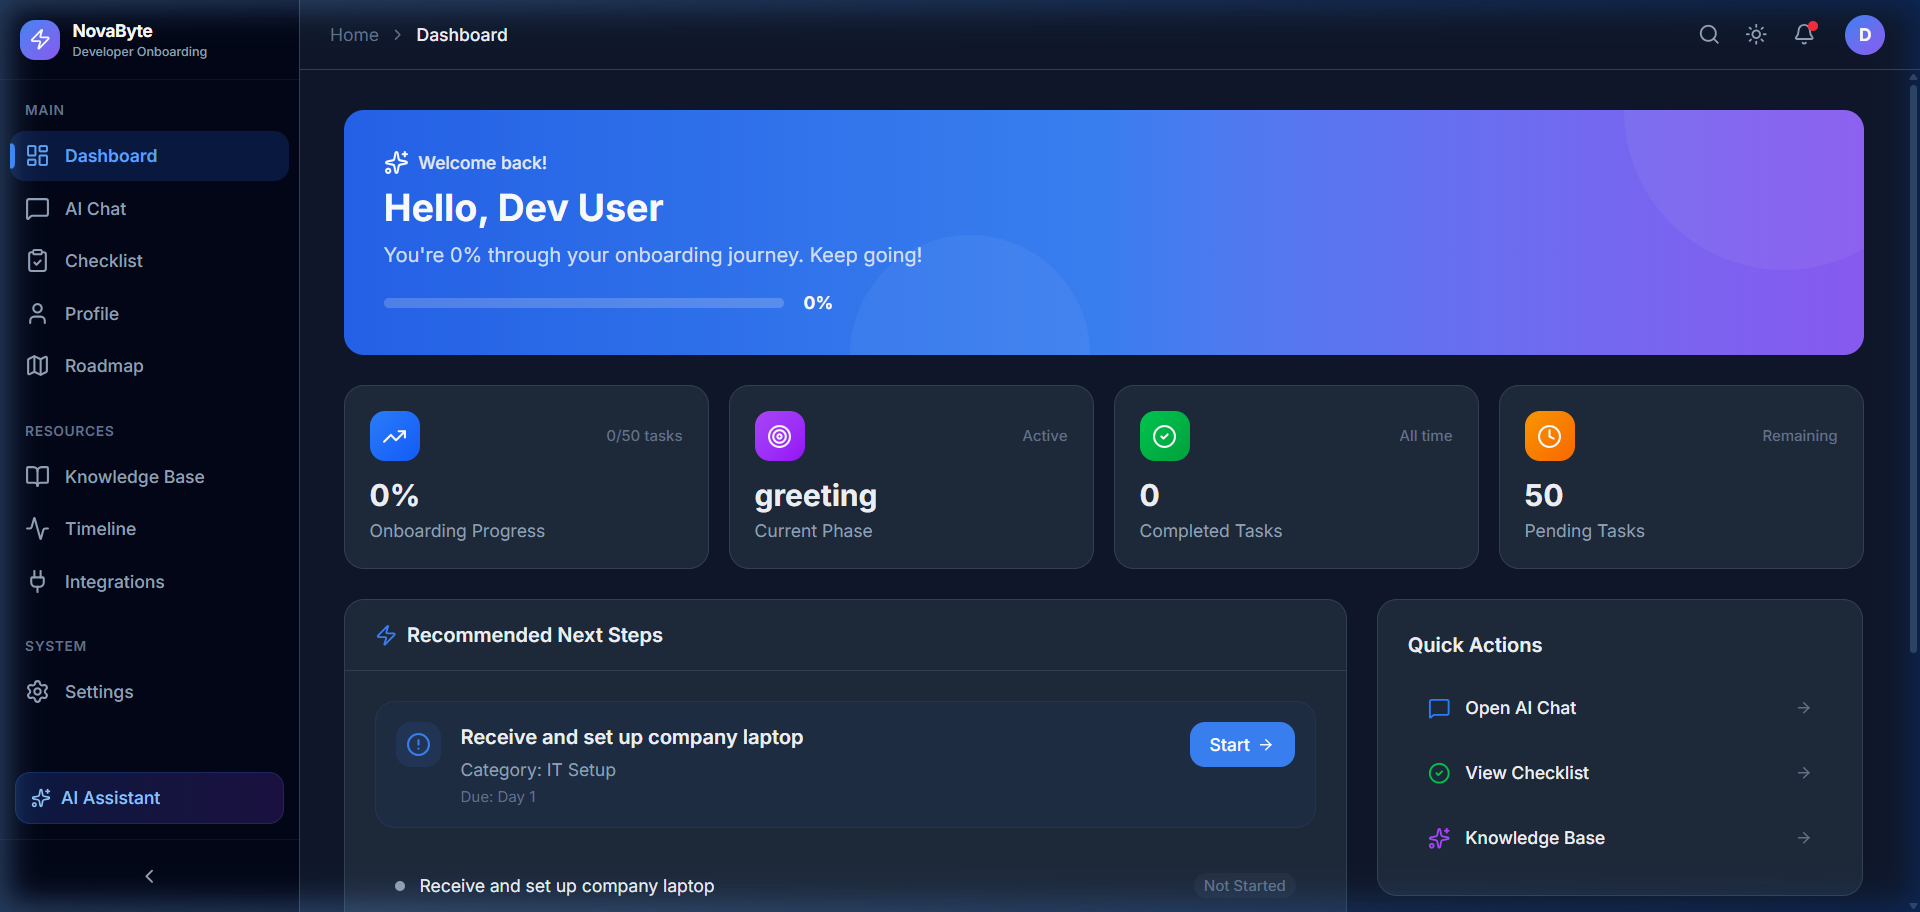
\includegraphics[width=0.85\textwidth]{figures/fig_dashboard.png}
\caption{NovaByte dashboard interface showing onboarding progress, task statistics, recommended next steps, and quick actions. The progress bar reflects real-time completion percentage computed from the checklist state.}
\label{fig:dashboard}
\end{figure*}

\begin{figure}[t]
\centering
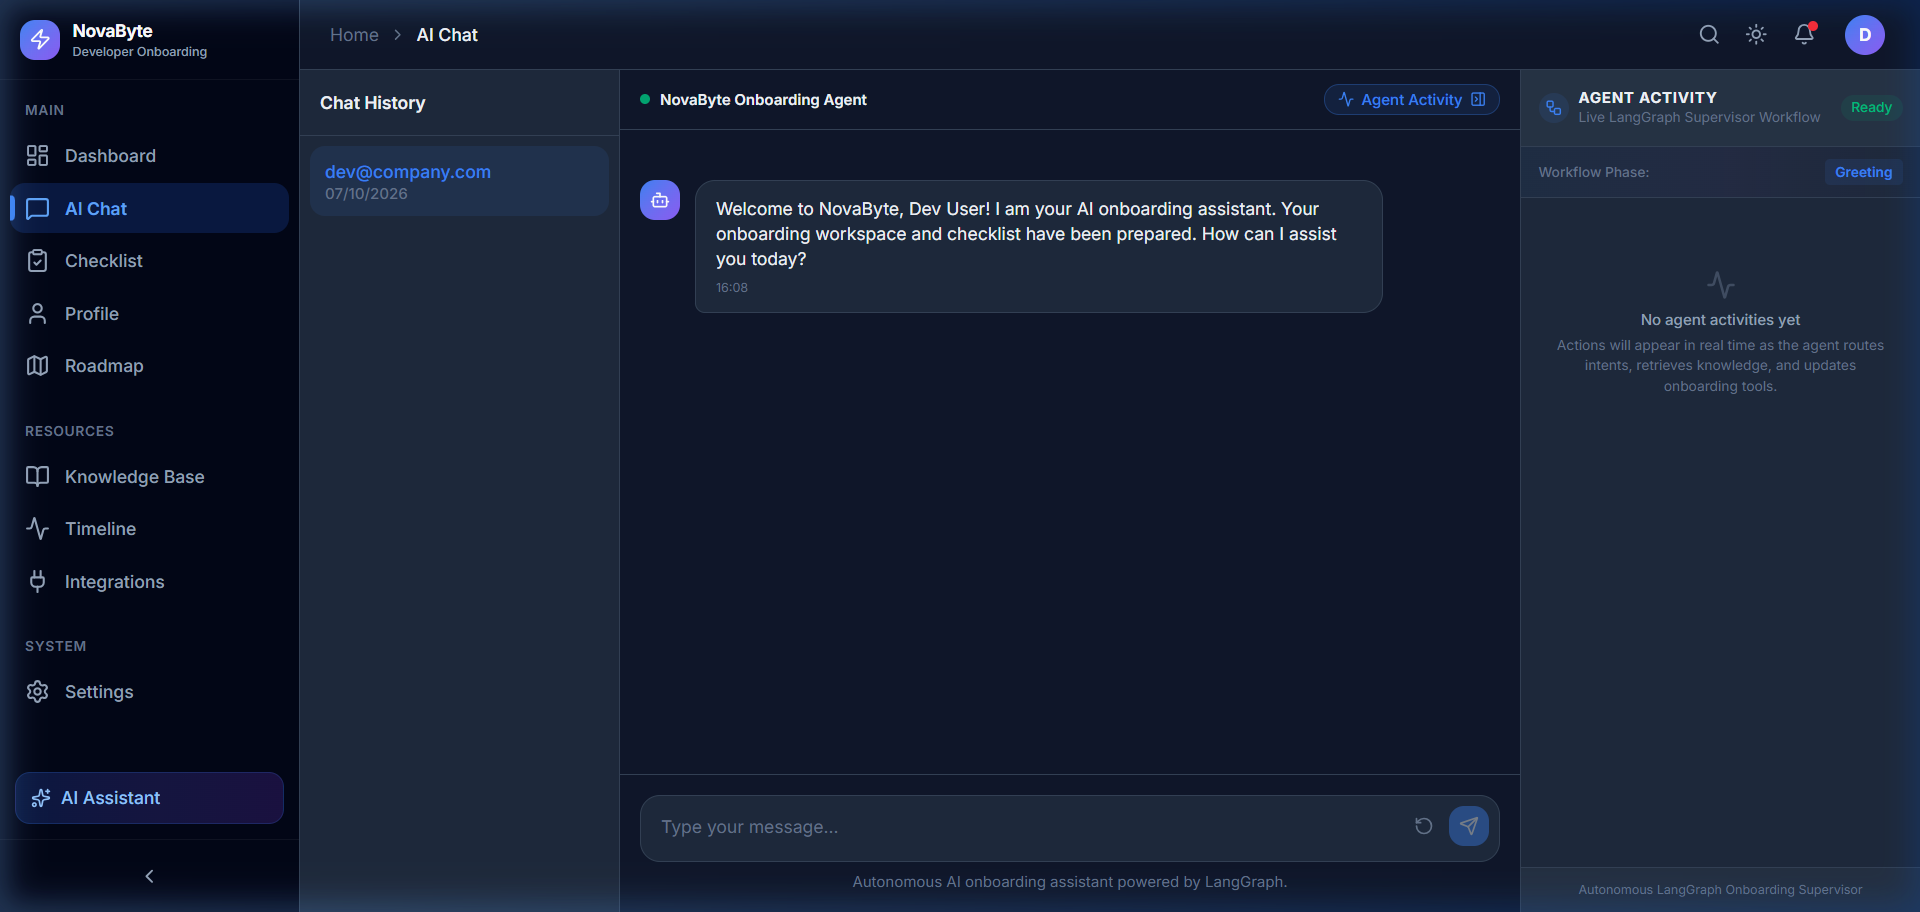
\includegraphics[width=\columnwidth]{figures/fig_chat.png}
\caption{AI Chat interface with conversational onboarding assistant. The right panel displays live LangGraph supervisor workflow activity, showing the current phase and real-time node execution status.}
\label{fig:chat}
\end{figure}

\begin{figure}[t]
\centering
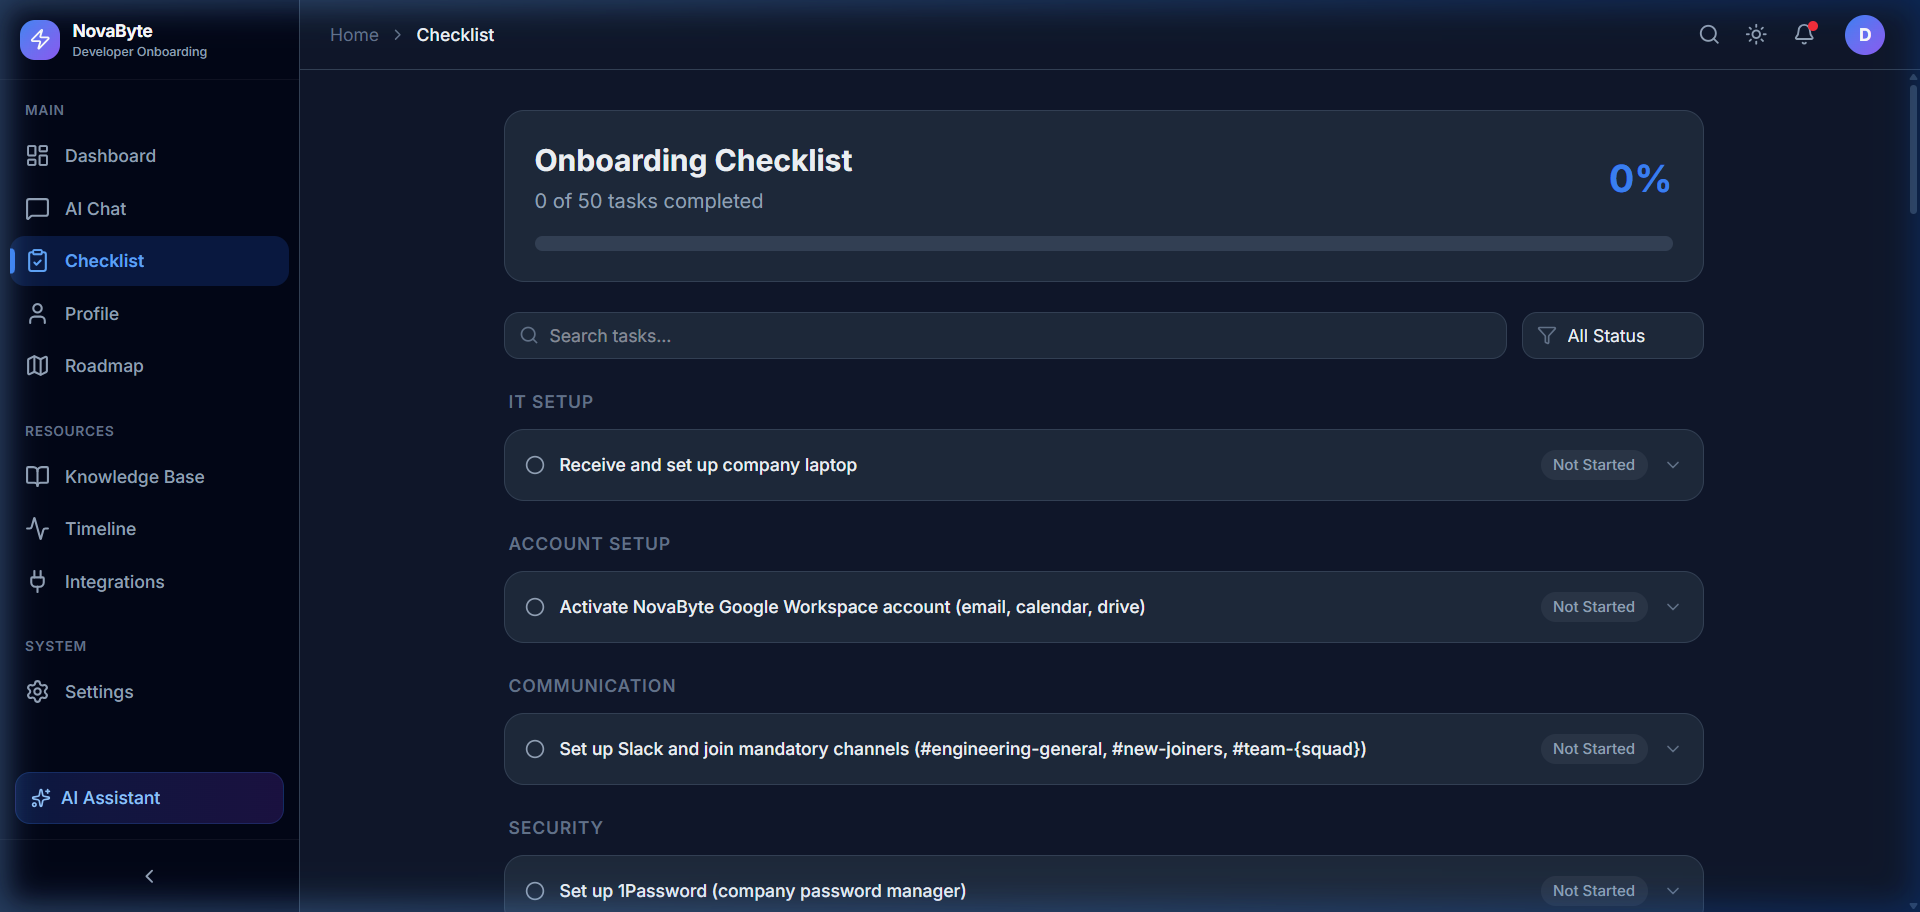
\includegraphics[width=\columnwidth]{figures/fig_checklist.png}
\caption{Onboarding checklist view with categorized tasks (IT Setup, Account Setup, Communication, Security), status filters, and real-time progress tracking.}
\label{fig:checklist}
\end{figure}

\begin{figure}[t]
\centering
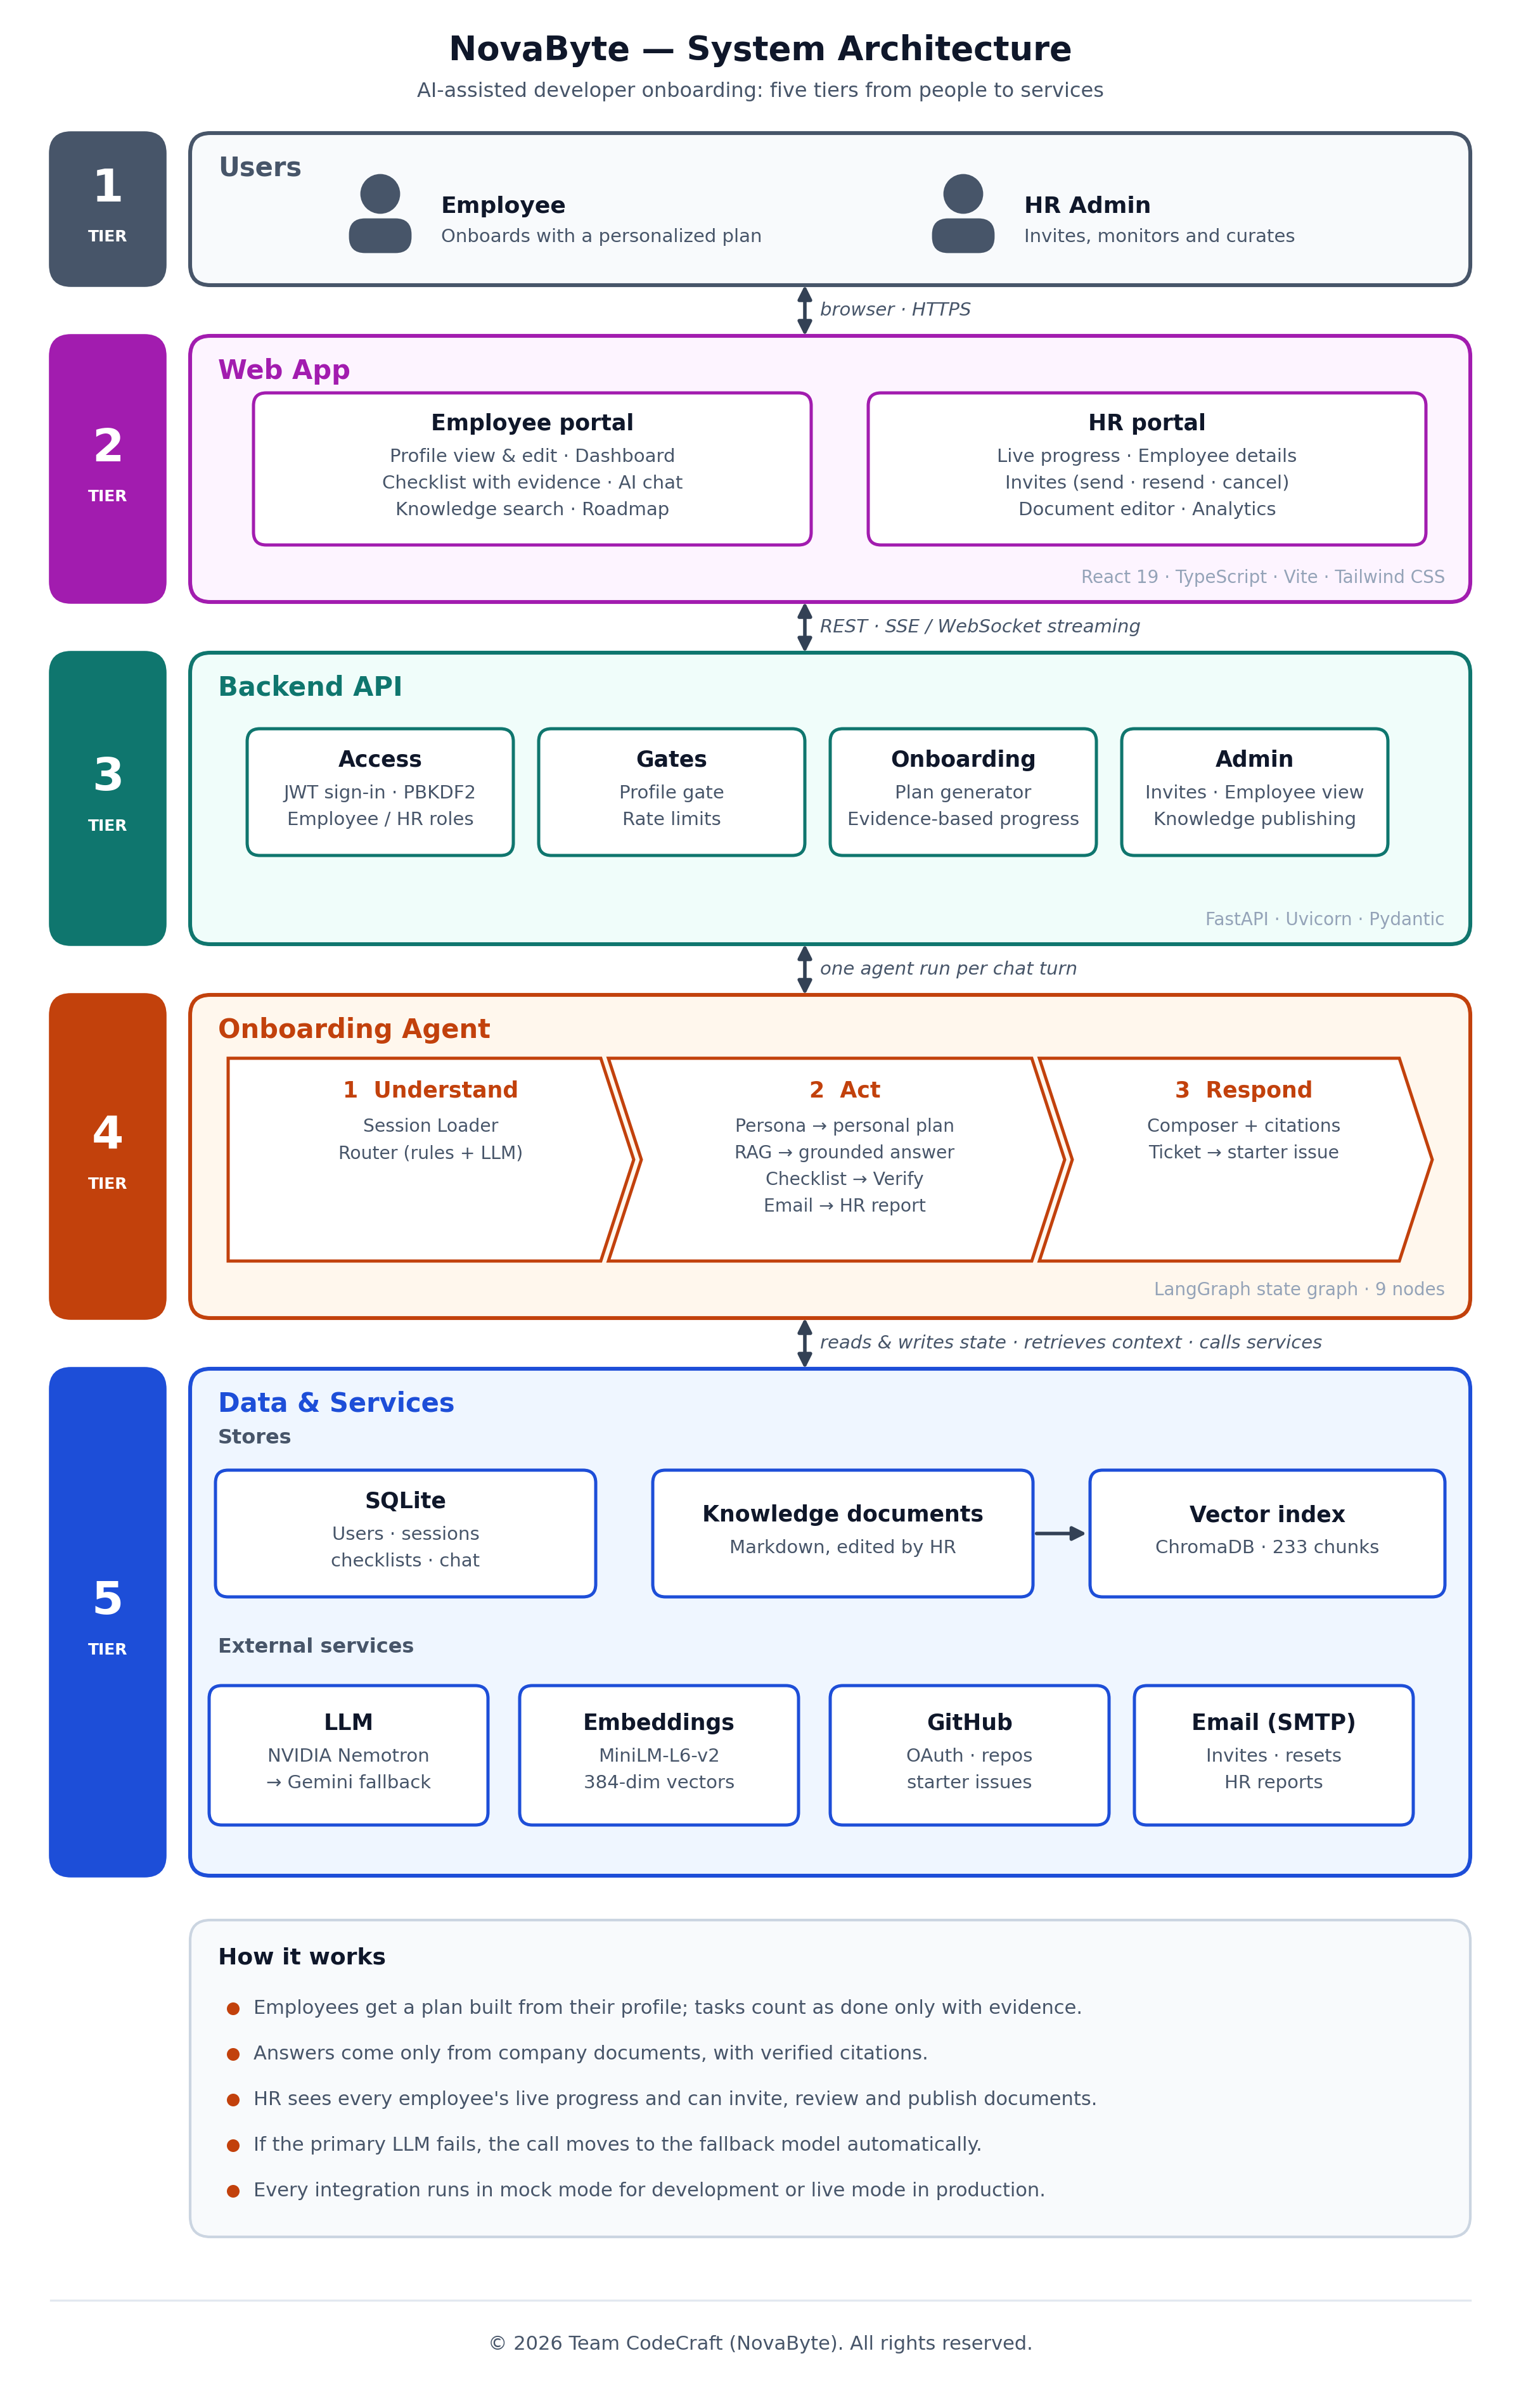
\includegraphics[width=\columnwidth]{figures/fig_architecture.png}
\caption{NovaByte system architecture in five tiers: Users (employee and HR administrator), Web App (employee and HR portals), Backend API, Onboarding Agent (nine LangGraph nodes grouped as Understand, Act, and Respond), and Data \& Services (SQLite, knowledge documents, vector index, LLM, embeddings, GitHub, SMTP). Diagram \textcopyright~2026 Team CodeCraft.}
\label{fig:architecture}
\end{figure}

\begin{figure}[t]
\centering
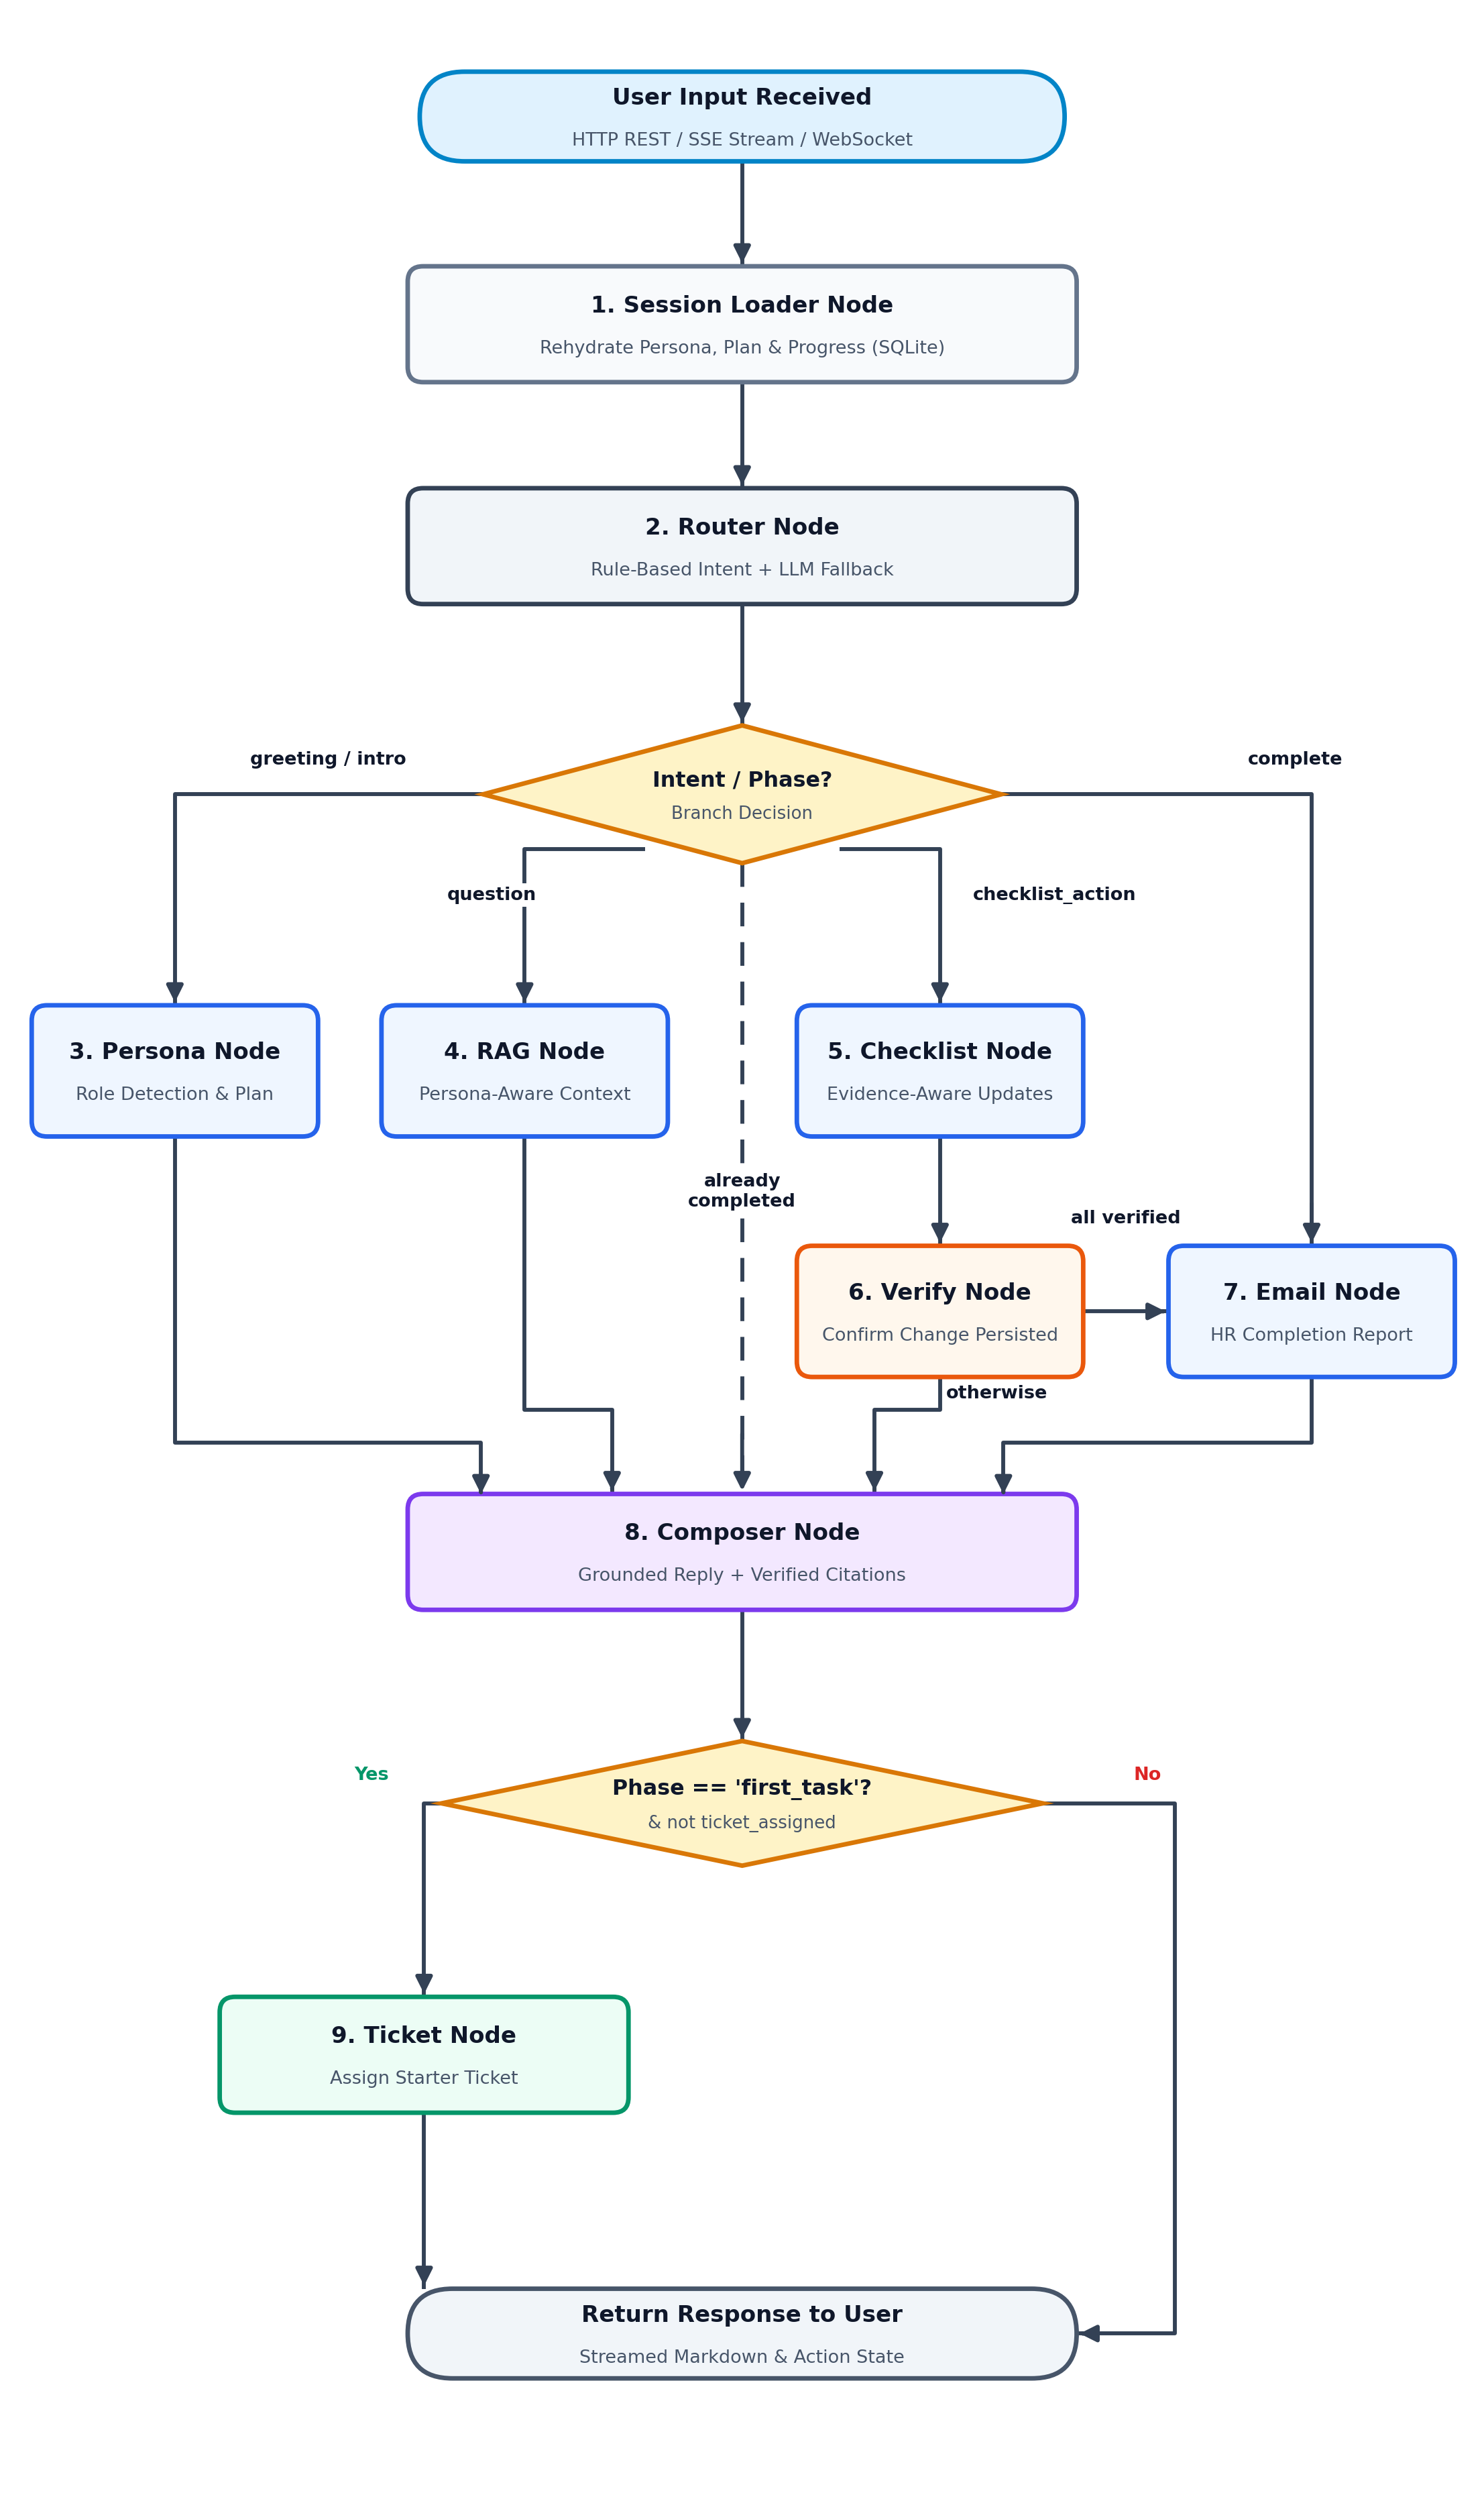
\includegraphics[width=\columnwidth]{figures/fig_workflow.png}
\caption{LangGraph agent workflow with nine processing nodes and conditional edge routing. The Router node classifies user intent and directs execution through specialized nodes before the Composer synthesizes the final response.}
\label{fig:workflow}
\end{figure}

\end{document}
